\documentclass[handout]{beamer}
%\documentclass [serif,mathserif,professionalfont]{beamer}
%\usepackage {pxfonts}
%\usepackage {eulervm}
%\usepackage{mathpazo}
%\logo{\includegraphics[height=1.2cm]{fsulogo.png}}

\usepackage{tikz}
\usepackage{graphicx}
\usepackage{subfig,fixltx2e,url}
\usepackage[latin1]{inputenc}
\usepackage{pgfplots}
\usepackage{hyperref}
\usepackage{booktabs}

%\usetheme{Warsaw}
\usecolortheme{lily}
\setbeamercovered{transparent}
%\useoutertheme[subsection=false]{smoothbars}

\setbeamertemplate{sidebar right}{}
\setbeamertemplate{footline}{%
\hfill\usebeamertemplate***{navigation symbols}
\hspace{1cm}\insertframenumber{}/\inserttotalframenumber}

\title[ \insertdate]{Multi-Input Multi-Output Electric Motor Modeling using Neural Networks}

\author{Sagar Verma}
\institute[Centralesup\'elec and Schneider Electric] % (optional, but mostly needed)
{
  Centre de Vision Num\'erique,\\
  Centralesup\'elec, Gif-sur-Yvette}
% - Use the \inst command only if there are several affiliations.
% - Keep it simple, no one is interested in your street address.

\date{December, 2018}
% - Either use conference name or its abbreviation.
% - Not really informative to the audience, more for people (including

\begin{document}

\begin{frame}
\titlepage
\end{frame}

\begin{frame}{Table Of Contents}
\begin{enumerate}
\item Dataset
\item Experiments
\item Results
\item Questions
\end{enumerate}
\end{frame}

\section{Problem Statement}

\begin{frame}{What we discussed in the last meeting?}
\begin{enumerate}
  \item Problem definition
  \item Neural networks introduction
  \item Early results on public dataset
  \item Error in predicting impulse peeks
  \item Prediction scaling problem
\end{enumerate}
\end{frame}


\begin{frame}{Dataset}{Description}
  \begin{enumerate}
    \item Single experiment
    \item 1200 seconds long
    \item Simulink dq-frame model is used
  \end{enumerate}
\end{frame}

\begin{frame}{Dataset}{Voltages}
\begin{center}
  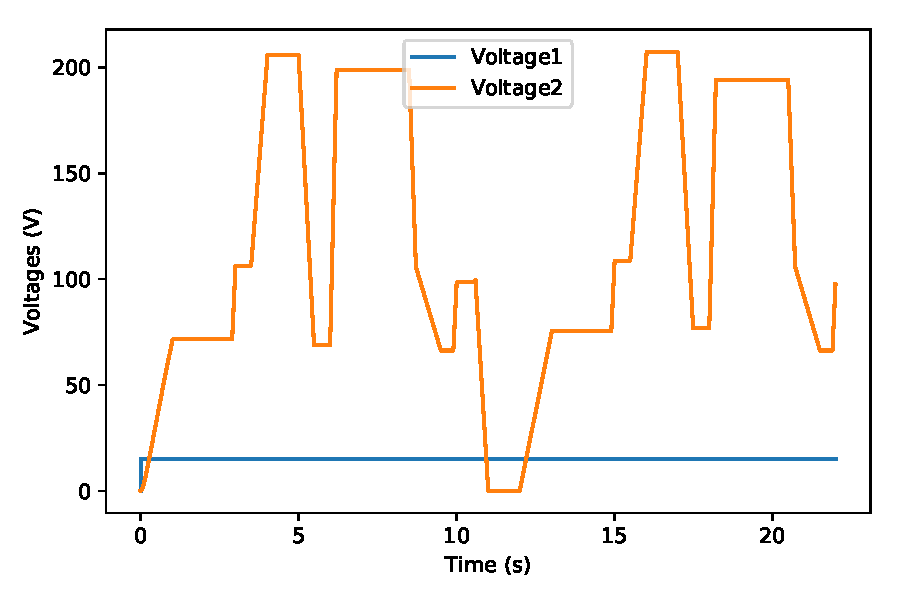
\includegraphics[scale=0.6]{images/voltages_vs_time}
\end{center}
\end{frame}

\begin{frame}{Dataset}{Stator Puls}
\begin{center}
  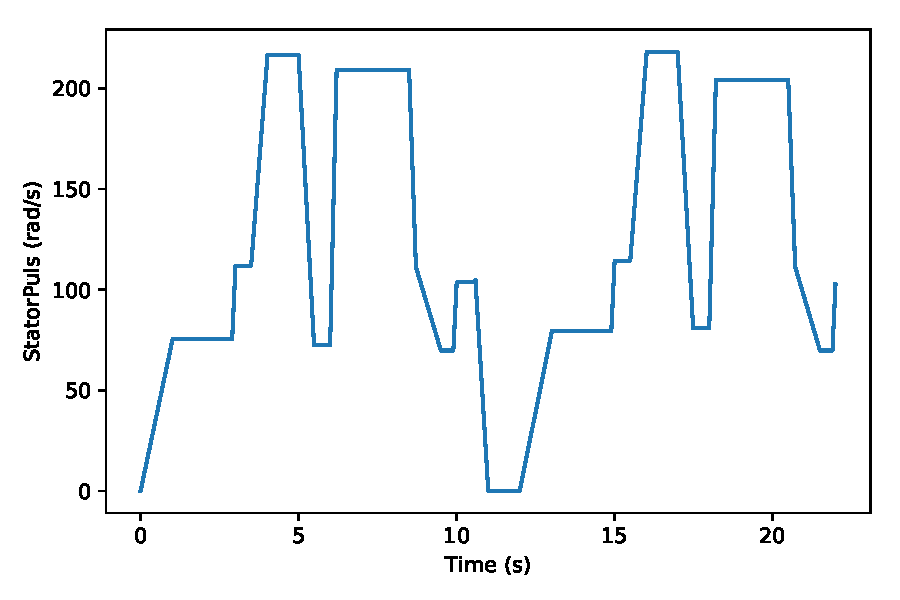
\includegraphics[scale=0.6]{images/statorpuls_vs_time}
\end{center}
\end{frame}

\begin{frame}{Dataset}{Speed}
\begin{center}
  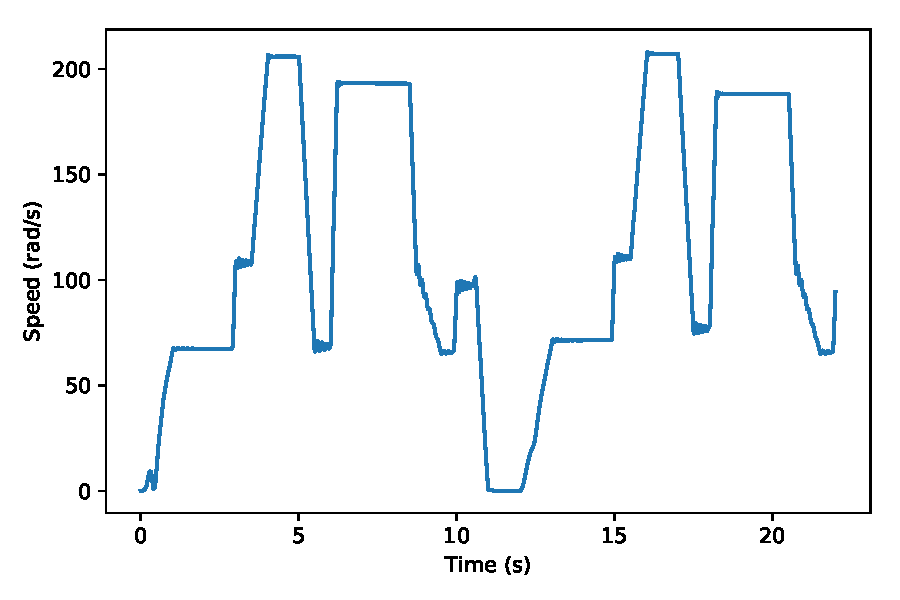
\includegraphics[scale=0.6]{images/speed_vs_time}
\end{center}
\end{frame}

\begin{frame}{Dataset}{Currents}
\begin{center}
  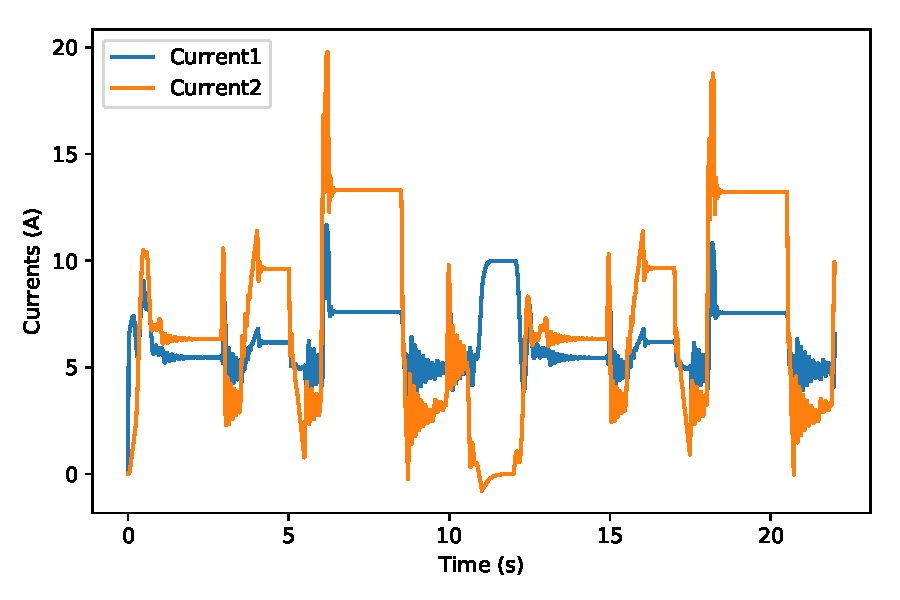
\includegraphics[scale=0.6]{images/currents_vs_time}
\end{center}
\end{frame}

\begin{frame}{Dataset}{Torque Load}
\begin{center}
  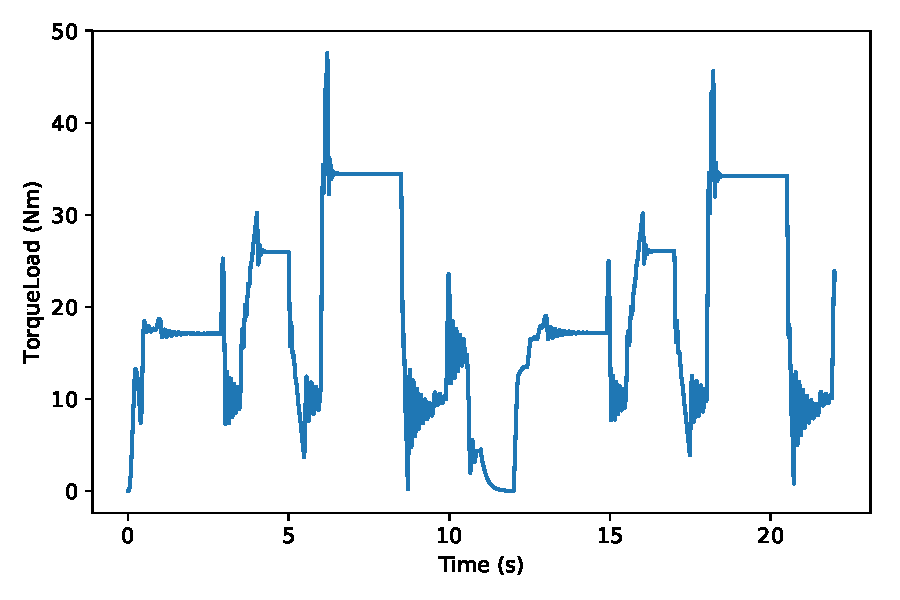
\includegraphics[scale=0.6]{images/torqueload_vs_time}
\end{center}
\end{frame}

\begin{frame}{Dataset}{Train-Test Split}
  \begin{enumerate}
    \item Single experiment
    \item Train on 0s-839s, test on 839s-1199.75s
    \item Window size $w=100$, stride $s=1$
  \end{enumerate}
\end{frame}

% \begin{frame}{Experiments}{ANN for signal prediction}
%   \begin{enumerate}
%     \item Three outputs, three networks.
%     \item Input: $w\times3$ 1-D vector, Output: $1$ middle value
%     \item Activation, $f$: Leaky Relu
%   \end{enumerate}
%   \begin{center}
%     \begin{figure}
%     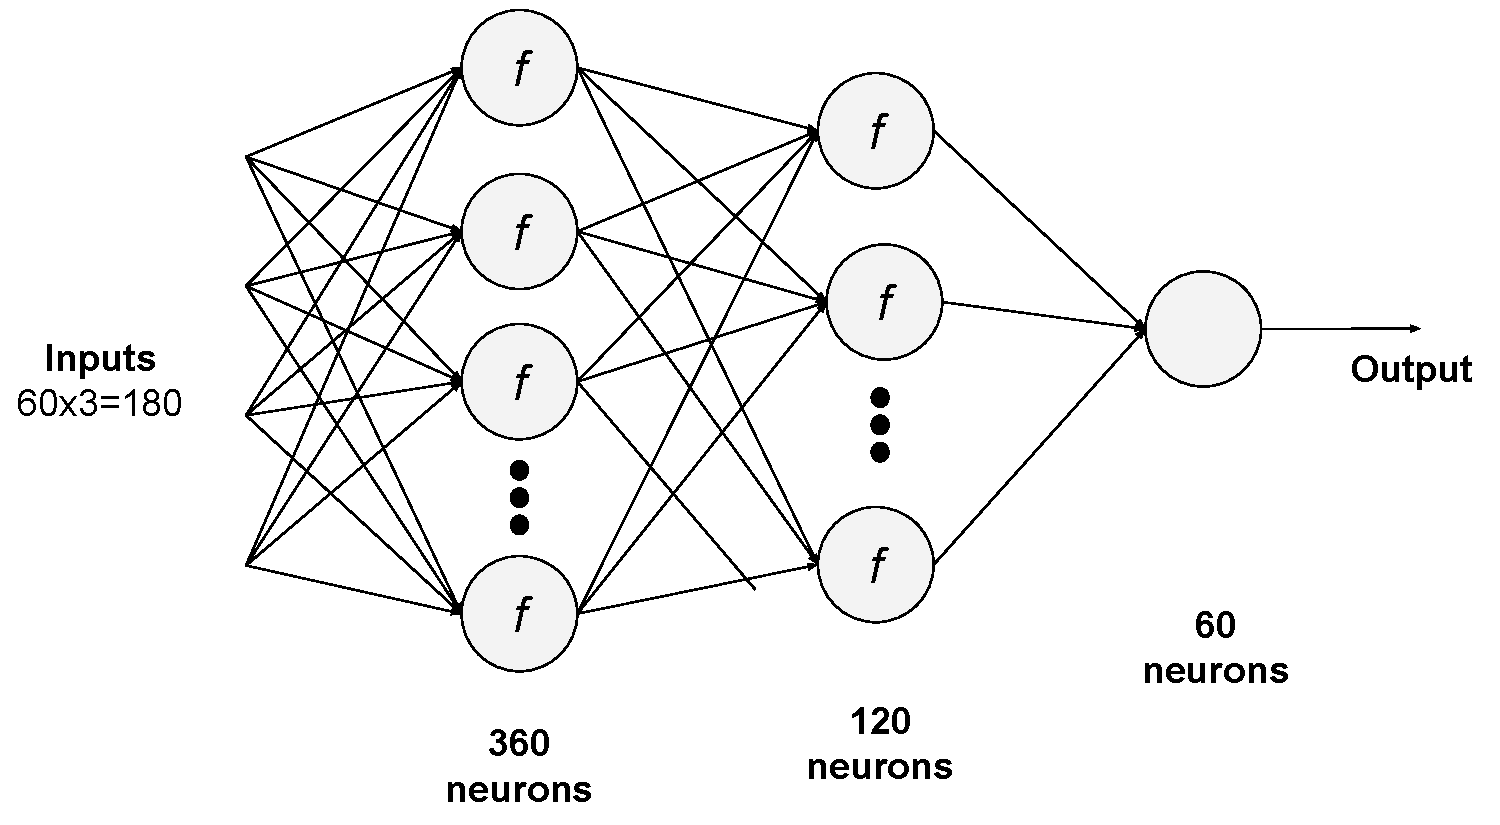
\includegraphics[scale=0.35]{images/motor_ann_1}
%     \end{figure}
%   \end{center}
% \end{frame}
%
% \begin{frame}{Experiments}{ANN with auxiliary task}
%   \begin{enumerate}
%     \item Also reconstruct input signal.
%     \item Three outputs, three networks.
%     \item Input: $w\times3$ 2-D vector, Output1: $1$, output2: $w\times3$ 2-D vector
%     \item Activation, $f$: Leaky Relu
%   \end{enumerate}
%   \begin{center}
%     \begin{figure}
%     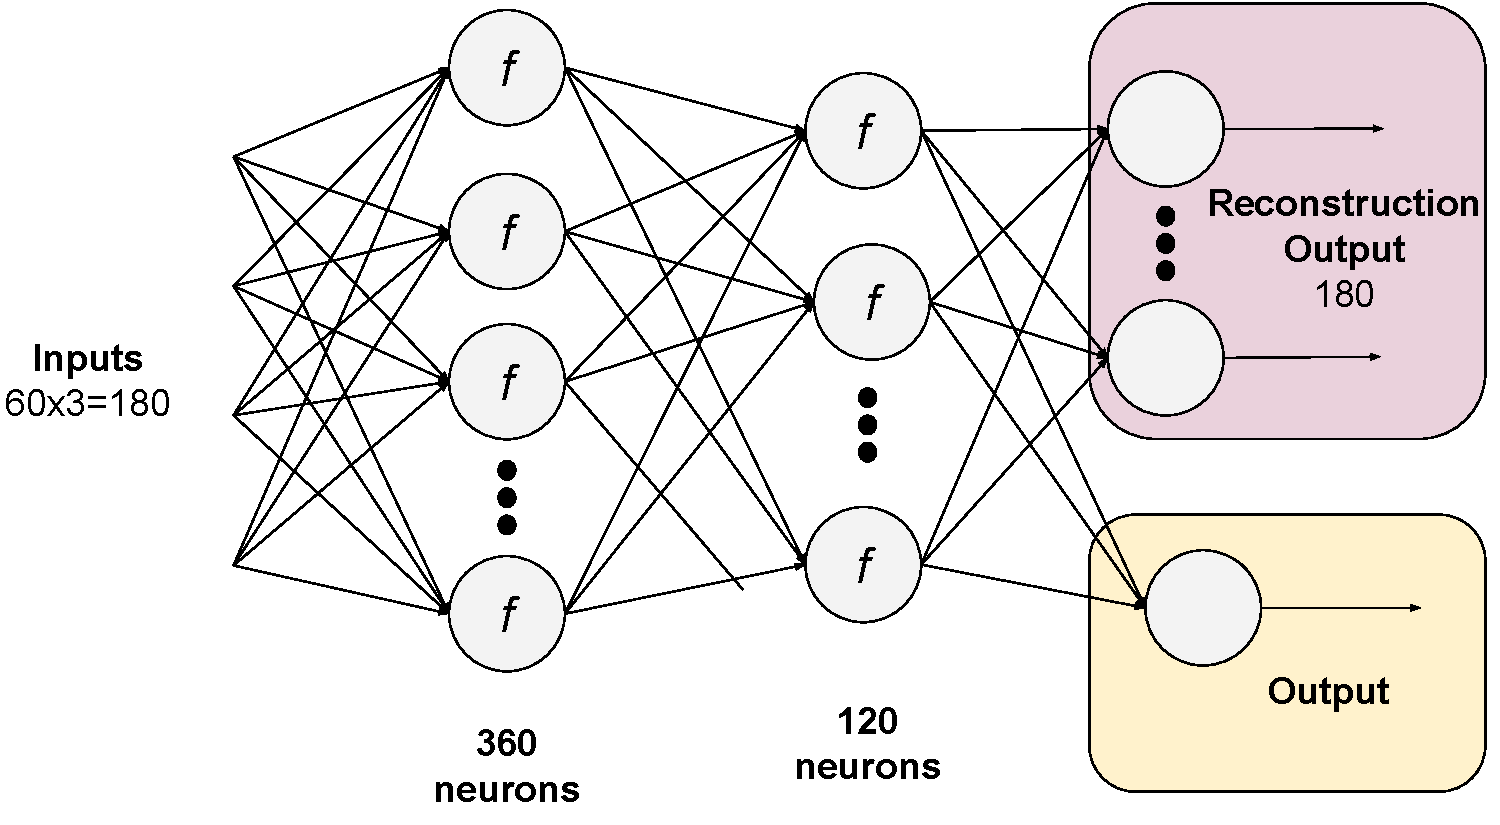
\includegraphics[scale=0.35]{images/motor_recon}
%     \end{figure}
%   \end{center}
% \end{frame}

\begin{frame}{Experiments}{Convolution network}
  \begin{enumerate}
    \item CNN and ANN works better then RNN (Miller et al. 2018).
    \item Encoder network
    \begin{enumerate}
      \item Kernels capture $w\leq10$
      \item Signals act as feature channels, no flattening
    \end{enumerate}
    \item Decoder network
    \begin{enumerate}
      \item Implicitly segment different temporal patterns
    \end{enumerate}
    \item Three outputs, three networks.
    \item Input: $w\times3$ 2-D vector, Output: $w$
  \end{enumerate}
\end{frame}

\begin{frame}{Convolution network}
\begin{center}
  \begin{figure}
  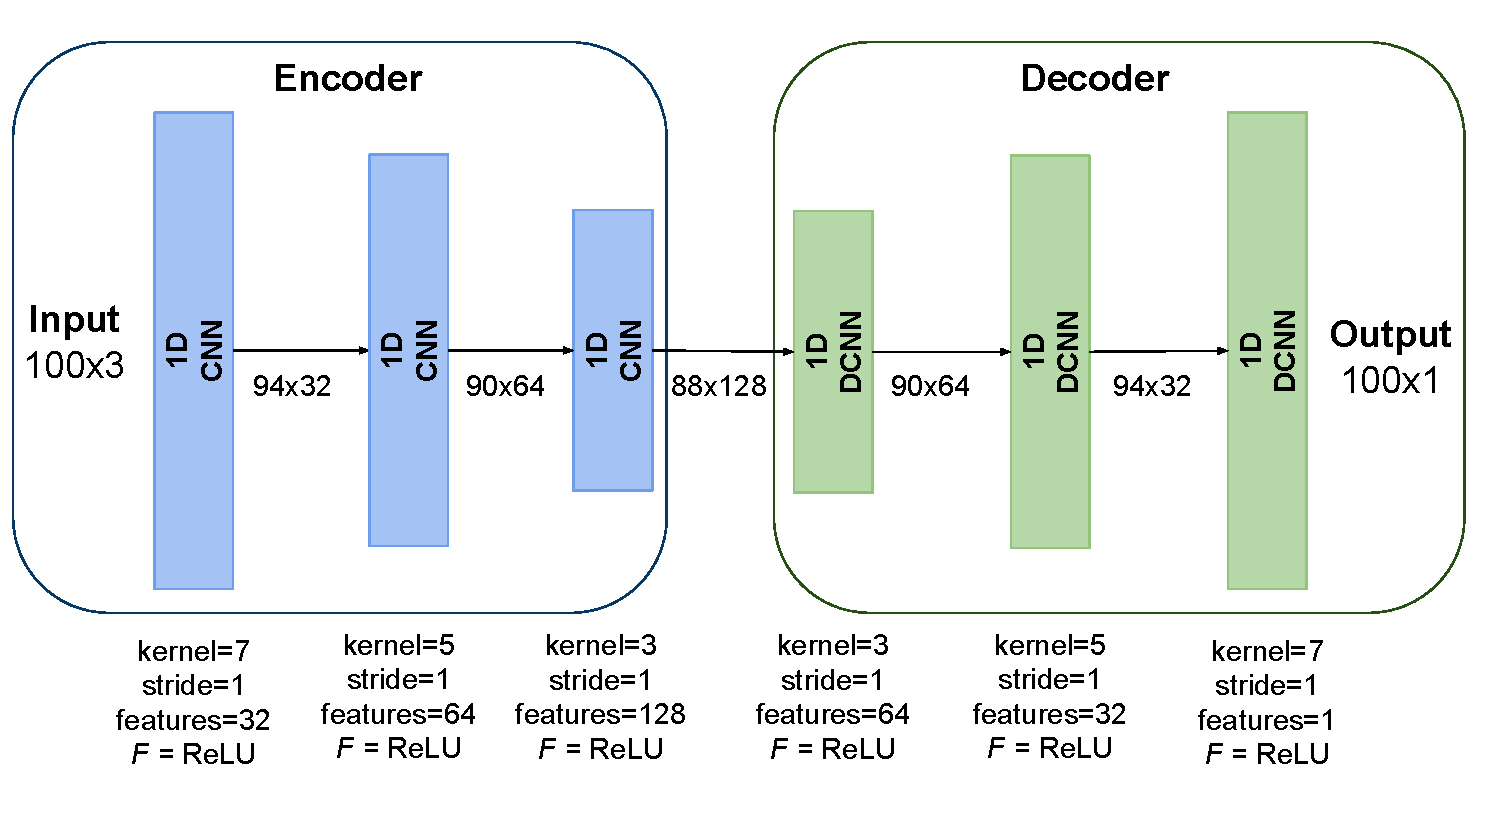
\includegraphics[scale=0.4]{images/motor_cnn_decoder_encoder}
  \end{figure}
\end{center}
\end{frame}

% \begin{frame}{Results}{Best Model}
% \begin{table}[]
%   \begin{tabular}{l c c c c}
%   \toprule[0.2mm]
%    \textbf{Model} & \textbf{w} & \textbf{Current1} & \textbf{Current2} & \textbf{Torque}\\
%    \midrule
%    \textbf{ANN} & 100 & 0.223 & 0.197 & 0.101 \\
%    \midrule
%    \textbf{ANN Aux} & 100 & 0.192 & 0.182 & 0.112 \\
%    \midrule
%    \textbf{CNN} & 100 & \textbf{0.107} & \textbf{0.104} & \textbf{0.091} \\
%    \bottomrule
%   \end{tabular}
%   \caption{MSE of different models.}
%   \end{table}
% \end{frame}
% \begin{frame}{RBM for signal prediction}
%
% \end{frame}

\begin{frame}{Results}{Current1}
\begin{center}
  \begin{figure}
  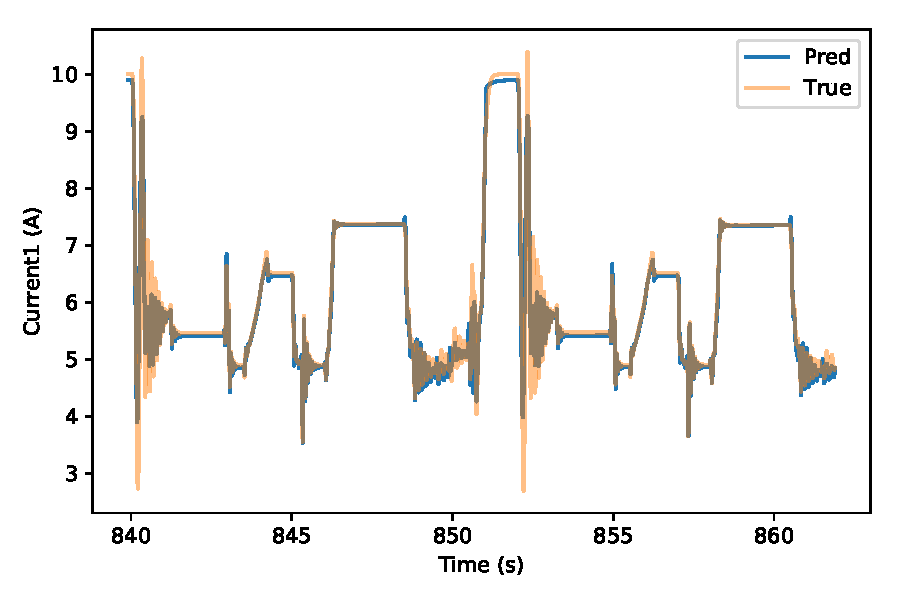
\includegraphics[scale=0.4]{images/current1_pred_vs_time} \\
  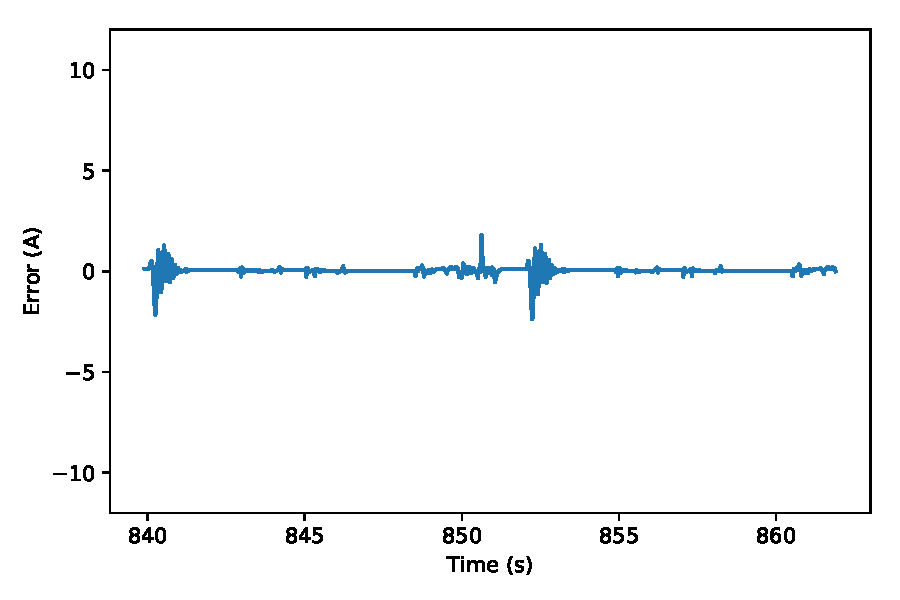
\includegraphics[scale=0.4]{images/current1_error_vs_time}
  \end{figure}
\end{center}
\end{frame}

\begin{frame}{Results}{Current2}
\begin{center}
  \begin{figure}
  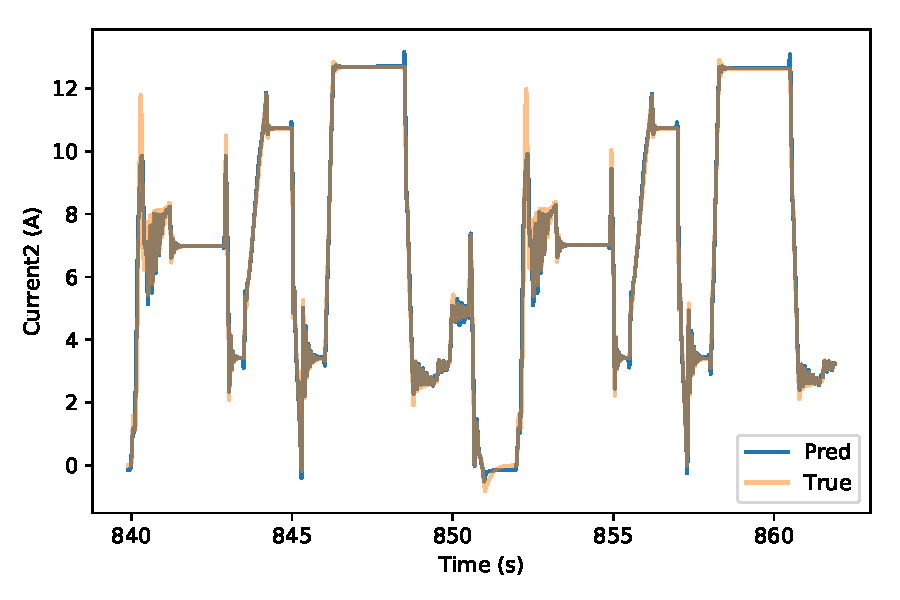
\includegraphics[scale=0.4]{images/current2_pred_vs_time}\\
 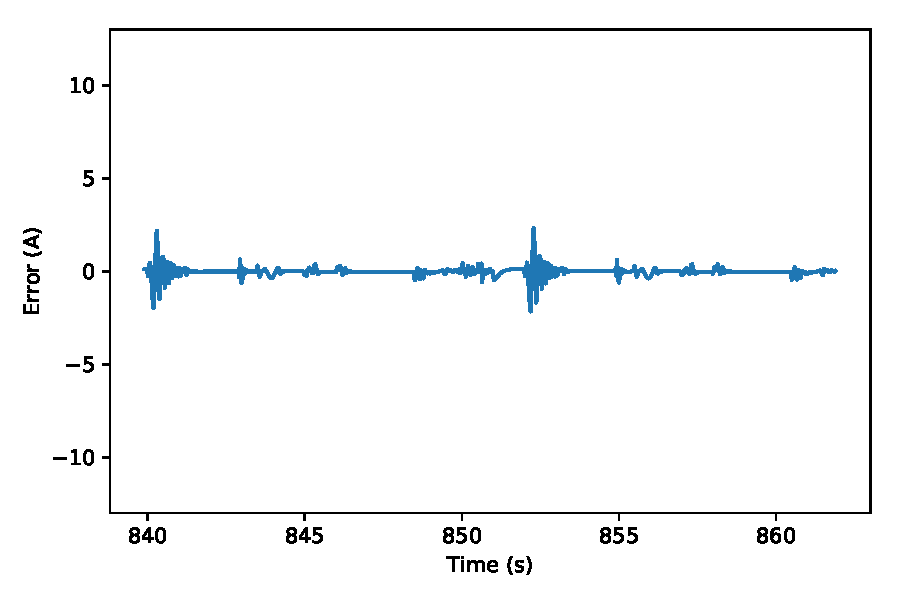
\includegraphics[scale=0.4]{images/current2_error_vs_time}
  \end{figure}
\end{center}
\end{frame}

\begin{frame}{Results}{Torque}
\begin{center}
  \begin{figure}
  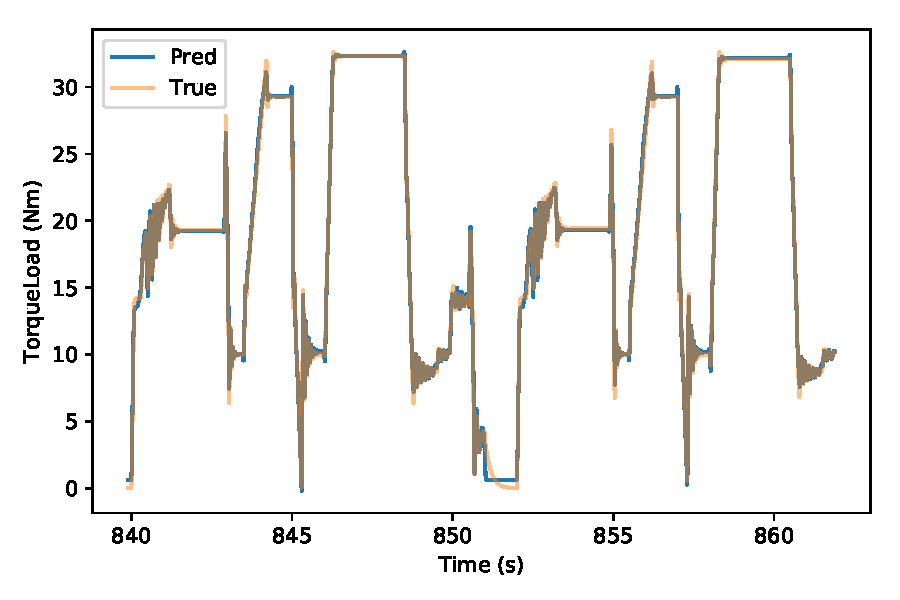
\includegraphics[scale=0.4]{images/torqueload_pred_vs_time} \\
  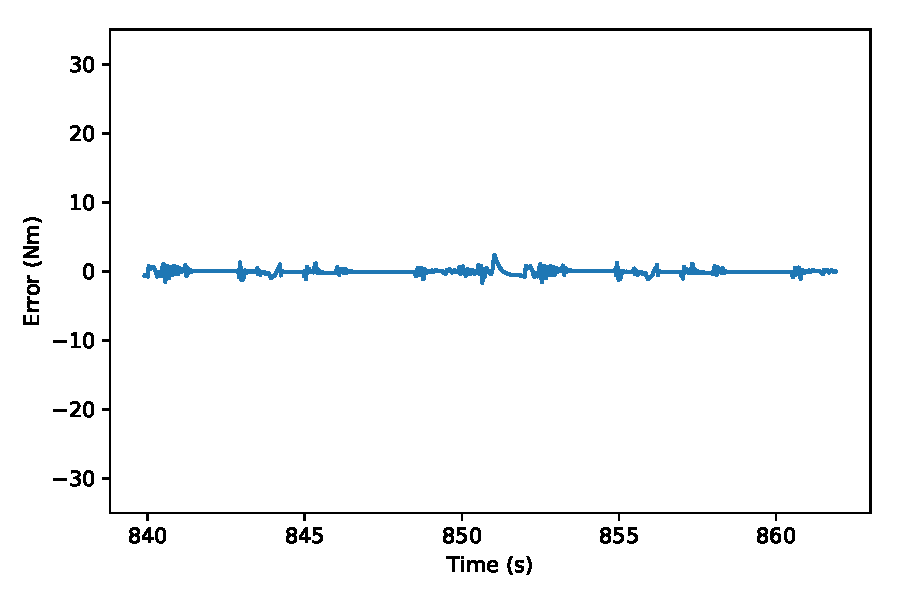
\includegraphics[scale=0.4]{images/torque_error_vs_time}
  \end{figure}
\end{center}
\end{frame}




% \section{Questions}
% \begin{frame}{Questions}
% \begin{enumerate}
%   \item Is data very simple?
%   \item When voltage 1 is not constant?
%   \item When Voltage 2 and stator pulse are not same?
%   \item Can signals be grouped into some classes?
%   \item Visual evaluations?
%   \item Other evaluation metrics?
%   \item Predict future(causal)?
% \end{enumerate}
% \end{frame}

\begin{frame}
\center
\color{blue}
\huge{Thank you!}\\
\end{frame}

\end{document}
